\begin{thm}{106}{\hosi 3\maru}{富山県立大 (2009)}
 $k$は定数で、$0<k<2$とする。直線 $y=kx$ と曲線 $y=\left|x^2-2x\right|$ で囲まれた2つの部分の面積が等しいとき、$k$の値を求めよ。
\end{thm}

曲線$y=\left|x^2-2x\right|$は、$x<0$, $x>2$のとき$y=x^2-2x$、$0\le x\le 2$のとき$y=-x^2+2x$と表される。$y=kx$と$y=\pm x^2\mp 2x$との交点の$x$座標は、$x=0, 2\pm k$ (複合同順) であることを踏まえると、直線$y=kx$と$y=\left|x^2-2x\right|$の交点の$x$座標は
\begin{align*}
x&=0, 2+k & k<-2, k\ge 2&\text{のとき} \\
x&=0 & -2\le k < 0&\text{のとき} \\
x&=0, 2 & k=0&\text{のとき} \\
x&=0, 2-k, 2+k & 0<k<2&\text{のとき}
\end{align*}
とまとめられる。囲まれた部分が2つとなるのは、$0<k<2$の場合のみであるから、以下$0<k<2$として考える。

\begin{figure}[H]
 \centering
 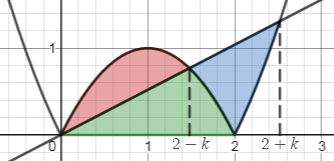
\includegraphics[width=0.7\linewidth]{../problems/Q_106/A_106.png}
\end{figure}
2つの領域は、上図の赤/青で示された領域となる。これらの面積が等しいためには赤$+$緑、と青$+$緑の面積が等しければよいので、
\begin{align*}
 \text{赤$+$緑} &= \int_0^2\! -(x^2-2x) \,dx = \frac{1}{6}(2^3-0^3)=\frac{4}{3} \\
 \text{青$+$緑} &= \int_{0}^{2+k}\!\! kx \,dx - \int_2^{2+k}\! (x^2-2x) \,dx \\
 &= \Bigl[\frac{1}{2}kx^2\Bigr]_0^{2+k} \!- \Bigl[\frac{1}{3}x^3-x^2\Bigr]_2^{2+k}=\frac{1}{6}(2+k)^3-\frac{4}{3}
\end{align*}
これらの面積が等しくなるような$k$は、
\begin{align*}
 \frac{1}{6}(2+k)^3-\frac{4}{3} &= \frac{4}{3} \\
 \dou\quad (2+k)^3&=16 \\
 \dou\quad k&=2\left(\sqrt[3]{2}-1\right)
\end{align*}
